\chapter{Auswertung}

Nach der Herstellung der bei einigen Proben ohne Zuhilfenahme von Hilfsmitteln das Vorhandensein der Gitterstruktur zu erkennen. Beim Betrachten der Proben unter bestimmten Winkeln war die Brechung des Lichtes durch das Gitter zu beobachten.

Eine Betrachtung der Proben unter dem Lichtmikroskop führte zu keinen Ergebnissen. Die Auflösung des Lichtmikroskops ist zu gering um die hergestellten Gitterstrukturen auflösen zu können (vgl. Abbildung \ref{fig:nix}). Gitterstrukturen mit einer Periode von 400~nm sind gerade noch vom Lichtmikroskop aufzulösen. Abbildung \ref{fig:400nm}\footnote[1]{Probe Hergestellt von Uwe Bog} zeigt ein solches Gitter unter 100-facher Vergrößerung.

\begin{figure}%
\centering
%\begin{adjustwidth}{0cm}{0cm}
	\subfloat[]{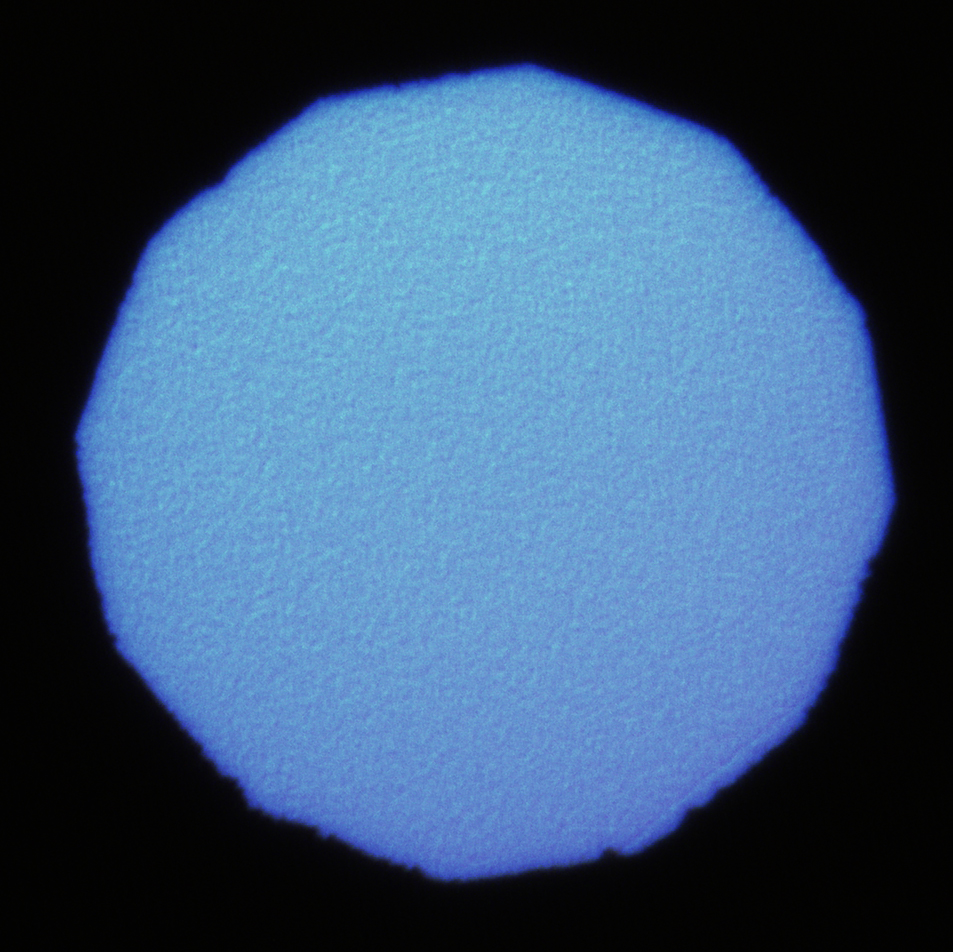
\includegraphics[totalheight=5 cm]{Grafiken/nix.jpg}\label{fig:nix}}\qquad
	\subfloat[]{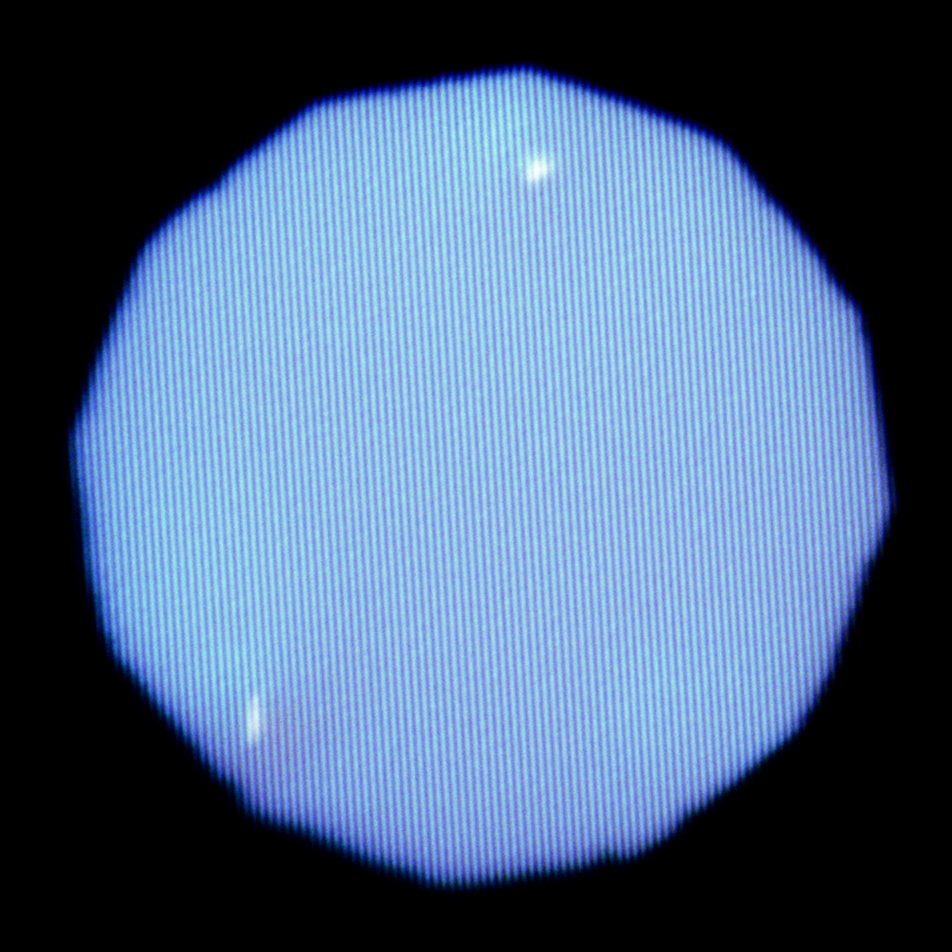
\includegraphics[totalheight=5 cm]{Grafiken/400nm.jpg} \label{fig:400nm}}\\%
%\end{adjustwidth}
\caption{Proben unter dem Lichtmikroskop. \textbf{(a)} Die Auflösung des Lichtmikroskops reicht nicht aus um die Strukturen aufzulösen. \textbf{(b)} Gitterstruktur mit einer Periodizität von 400~nm.$^1$}%
\label{fig:matlab}%
\end{figure}



Um die hergestellten Proben zu Charakterisieren wurden die Proben am Institut für Mikrosystemtechnik (IMT) mit einem \textit{Atomic Force Microscope} (AFM) vermessen. Abbildung \ref{fig:3d_bild} zeigt die mit dem AFM Topografie einer hergestellten Gitterstruktur.

\begin{figure}%
\centering
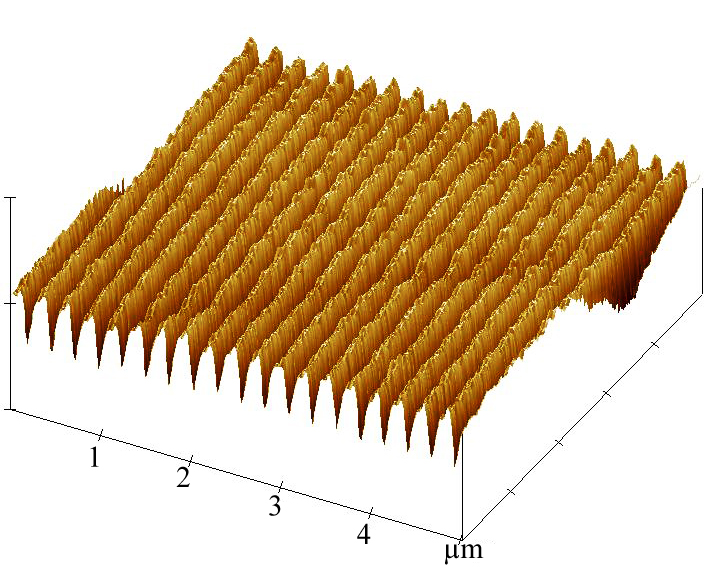
\includegraphics[width=.5\columnwidth]{Grafiken/3d_bild.jpg}%
\caption{AFM Messung der Topografie einer hergestellten Gitterstruktur (40~mJ, 4~s Entwicklungszeit).}%
\label{}%
\end{figure}


Im Folgenden sollen die Auswirkungen der Belichtungsdosis und der Entwicklungszeit auf die hergestellten Gitterstrukturen untersucht werden. Hierzu werden neben den im Rahmen des Laborversuches hergestellten Proben (vgl. Tabelle \ref{tab:parameter}) auch weitere Proben verwendet. Diese wurden im Labor Nanotechnologie von Matthias Baßler, Simon Jauß und Martin Waldvogel unter Anleitung von Uwe Bog hergestellt und vermessen wurden.\footnote[2]{Baßler, Jauß, Waldvogel; Präsentation zum Laboversuch Laser Interverenz Lithographie; 15.08.2011} Tabelle \ref{tab:Referenz} zeigt die Parameter dieser Proben.

\begin{table}[h]%
\centering
\caption{Von Laborgruppe ''Baßler``$^2$ hergestellte Proben.}
\begin{tabular}{cc}

\toprule
Entwicklungsdauer	& Belichtungsenergien\\
in s	& in mJ\\
\midrule
10 & 10, 40, 80\\
20  & 10, 40, 80\\
30 & 10, 40, 80\\
\bottomrule 
\end{tabular}
\label{tab:Referenz}
\end{table}

